\documentclass[svgnames]{beamer}

\usepackage[utf8]{inputenc}
\usepackage[T1]{fontenc}
\usepackage[french]{babel}
\usepackage{float}
\usetheme{Frankfurt}
\usepackage{enumitem}
\usepackage{pifont}
\usepackage{xcolor}
\usepackage{graphicx}
\usepackage{relsize}
\usepackage{array}
\usepackage{multirow}
\usepackage{multicol}
\usepackage{pgf, tikz}
\usetikzlibrary{arrows,shapes,positioning}
\usepackage{adjustbox}
\usepackage{makecell}
\usepackage[style=authoryear]{biblatex}
\usepackage{framed}
\usepackage{listings}

\def\checkmark{\tikz\fill[scale=0.4](0,.35) -- (.25,0) -- (1,.7) -- (.25,.15) -- cycle;}

\newenvironment{subitemize}{%
    \smaller
    \itemize
}{%
    \enditemize
}


%\setbeamertemplate{navigation symbols}{%
%	\insertframenumber/\inserttotalframenumber
%}
%
%\setbeamertemplate{headline}{%
%\leavevmode%
%  \hbox{%
%    \begin{beamercolorbox}[wd=\paperwidth,ht=2.5ex,dp=1.125ex]{palette quaternary}%
%    \insertsectionnavigationhorizontal{\paperwidth}{}{\hskip0pt plus1filll}
%    \insertsubsectionnavigationhorizontal{\paperwidth}{}{\hskip0pt plus1filll}
%    \end{beamercolorbox}%
%  }
%
%}

\definecolor{myblue}{cmyk}{1,.72,0,.38}
\definecolor{myblue2}{cmyk}{1,.65,0,.28}

\setbeamertemplate{bibliography item}{\insertbiblabel}

\newcommand{\mycite}[1]{[\textit{\cite{#1}}]}

\newcommand{\mypart}[1]{\part{#1}\begin{frame}\tableofcontents\end{frame}}
%\AtBeginPart[]
%{
%  \begin{frame}
%  \frametitle{\secname}
%  %\begin{multicols}{2}
%  \tableofcontents[hideallsubsections]
%  %\end{multicols}
%  \end{frame}
%}

\addbibresource{biblio.bib}



\title[]{Contribution à l'apprentissage humain de gestes à l'aide de techniques de clustering pour l’analyse de mouvements capturés}
\author{Quentin Couland}
\institute{}
\date{\today}

\setbeamerfont{subsection in toc}{size=\small}
\setbeamerfont{subsection in toc}{size=\smaller}


\begin{document}

	\maketitle

	\part{Cadre}
	\section{Cadre de la thèse}
	\begin{frame}{\subsecname}
	\centering
		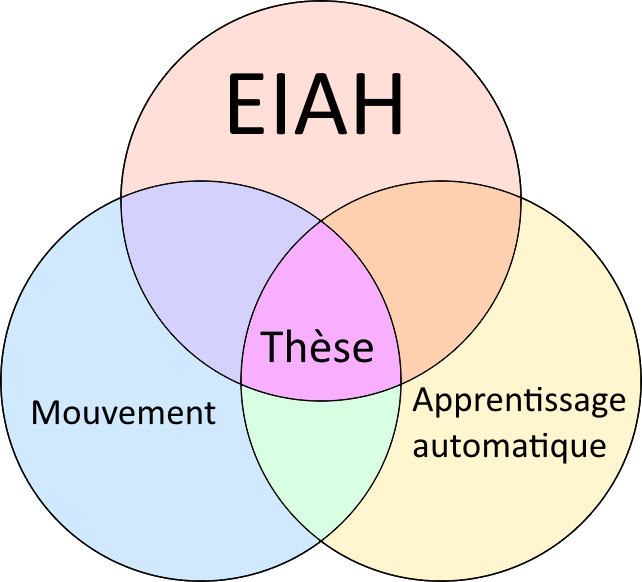
\includegraphics[scale=0.5]{img/venn_cadre.png}
	\end{frame}

	\begin{frame}{\secname}
	    \begin{block}{EIAH \mycite{Tchounikine2009PdR}}
	    « Environnements ayant pour but de favoriser l'apprentissage, en aidant, guidant et évaluant les apprenants d'une part et en assistant les enseignants d'autre part : que ce soit en présentiel, à distance, ou en situation mixte. »
	    \end{block}

	\begin{block}{Mouvement}
		\begin{center}
			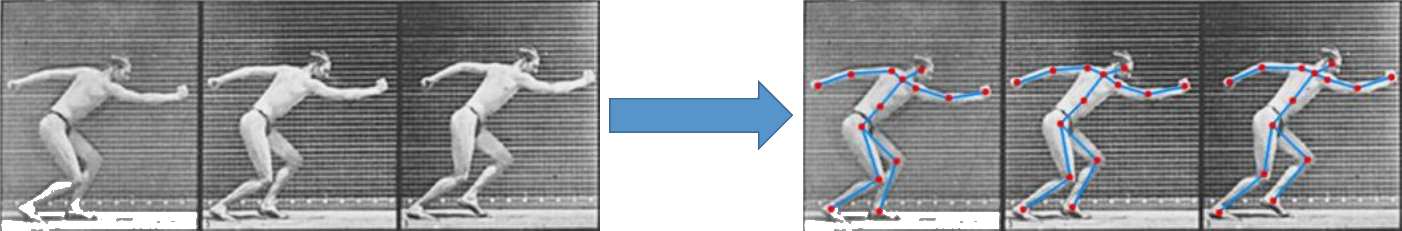
\includegraphics[scale=0.35]{img/mouvement_cadre_2.png}
		\end{center}
	\end{block}
		
		
		\begin{block}{Apprentissage automatique}
		Plusieurs familles d'algorithmes d'apprentissage automatique : Apprentissage supervisé / non-supervisé / semi-supervisé
		\end{block}
	\end{frame}
	
	\section{Problématique de la thèse}
	\begin{frame}{Problématique}
		Quelles sont les facteurs limitant à la réalisation d'un EIAH dédié à l'apprentissage humain de gestes, utilisable dans plusieurs domaines différents ?\\
		
		4 verrous identifiés :
		\begin{itemize}
			\item Analyse fine des mouvements
			\item Formalisation de l'expertise
			\item Visualisation d'indicateurs intelligibles
			\item Restitution sous forme de conseils adaptés
		\end{itemize}
	\end{frame}
	
	\section{Questions de recherche}
	\begin{frame}{\secname}
		\begin{itemize}[label=$-$]
			\item \textbf{Q1} : Comment développer un système permettant de caractériser le geste à l'aide de l'intégration de l'expertise d'un enseignant?
			\item \textbf{Q2} : Comment évaluer et comparer le geste (ou ses propriétés) de l'apprenant avec celui de l'enseignant afin d'évaluer la progression de l'apprentissage?
			\item \textbf{Q3} : Comment, dans une situation d'apprentissage de gestes donnée, proposer des retours pertinents et compréhensibles aux acteurs de l'apprentissage non spécialistes en analyse du mouvement?
		\end{itemize}
	\end{frame}

	
	
	\mypart{Etat de l'art}
	\section{EIAH pour l'apprentissage du geste}
	\begin{frame}{\secname}
		De nombreux EIAH aux finalités différentes :
		\begin{itemize}[label=$\bullet$]
			\item Rééducation \mycite{Alankus2010TCG}
			\item Amélioration de la performance sportive \mycite{Baldominos2015AAt}
			\item etc.
		\end{itemize}
		
		Mais également dans des domaines variés :
		\begin{itemize}[label=$\bullet$]
			\item Médical (analyse de postures \mycite{Aminian2004Chm}, chirurgie \mycite{BMT_2015}, etc.)
			\item Sport (danse \mycite{Maes2012DtM}, archerie japonaise \mycite{Yoshinaga2015Doa}, lancer de disques \mycite{YAMAOKA2013912}, etc.)
		\end{itemize}
	\end{frame}
	
	\begin{frame}{\secname}
		\centering
		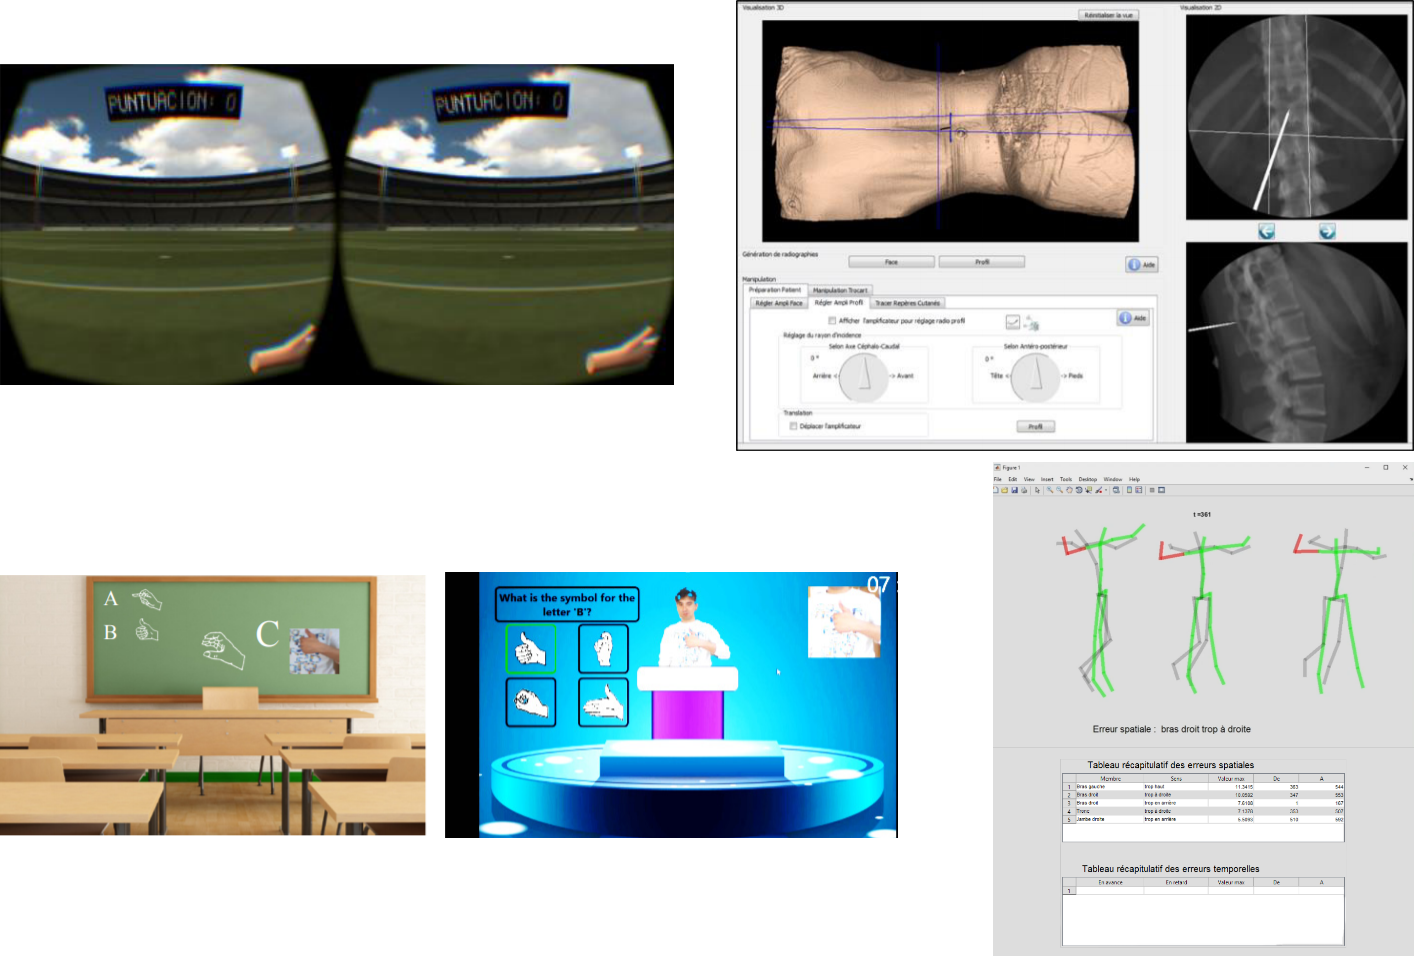
\includegraphics[scale=0.3]{img/all_eiah.png}
	\end{frame}
	
	\begin{frame}{Limites récurrentes}
		\centering
		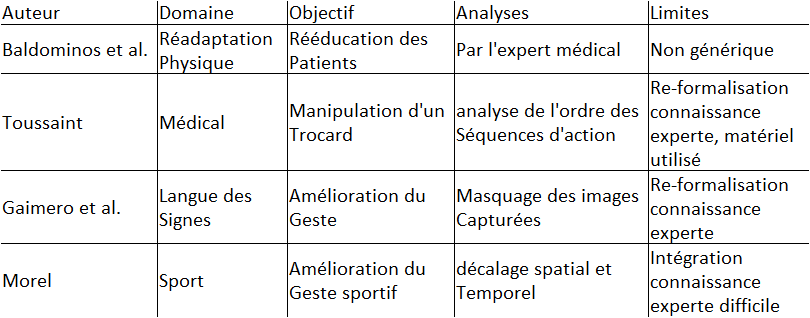
\includegraphics[scale=0.5]{img/tableau_eiah_2.png}
	\end{frame}
	
	\section{Analyse du mouvement capturé}
	\subsection{Descripteurs du descripteurs}
	\begin{frame}{\subsecname}
		\begin{block}{Descripteur du mouvement}
			Un descripteur est un indicateur calculé à partir du mouvement brut :  « Des observables signifiant sur le plan pédagogique » calculés à partir de traces (tous types de données, générées à partir des interactions de l’étudiant avec le système) ou d’autres indicateurs \mycite{Choquet2007MTf}
		\end{block}
	\end{frame}
	
	\subsection{Analyse par observation humaine}
	\begin{frame}{\subsecname}
		\begin{itemize}[label=$\bullet$]
			\item Visualisation de la performance de l'apprenant \mycite{Burns2011Uvh}
			\item Superposition de l'apprenant à un ou des modèles expert \mycite{Yoshinaga2015Doa}
		\end{itemize}
		\centering
			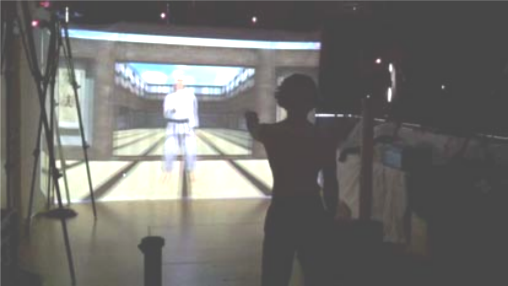
\includegraphics[scale=0.4]{img/Burns_karate.png}
			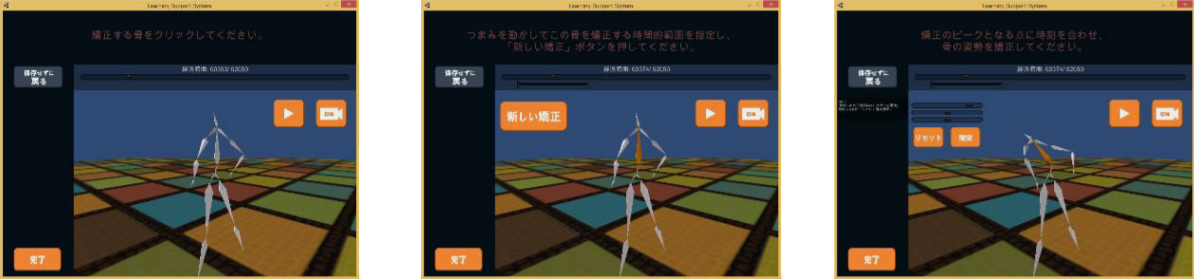
\includegraphics[scale=0.4]{img/Yoshiniga_archery.png}
	\end{frame}
	
	\subsection{Analyse par observation d'indicateurs}
	\begin{frame}{\subsecname}
		\begin{itemize}[label=$\bullet$]
			\item Positions relatives des parties du corps à des moments clés du lancer \mycite{Yamaoka2013FoF}
			\item Décomposition du mouvement à l'aide d'un seul descripteur \mycite{Kyan2015ABD}
			
			\centering
				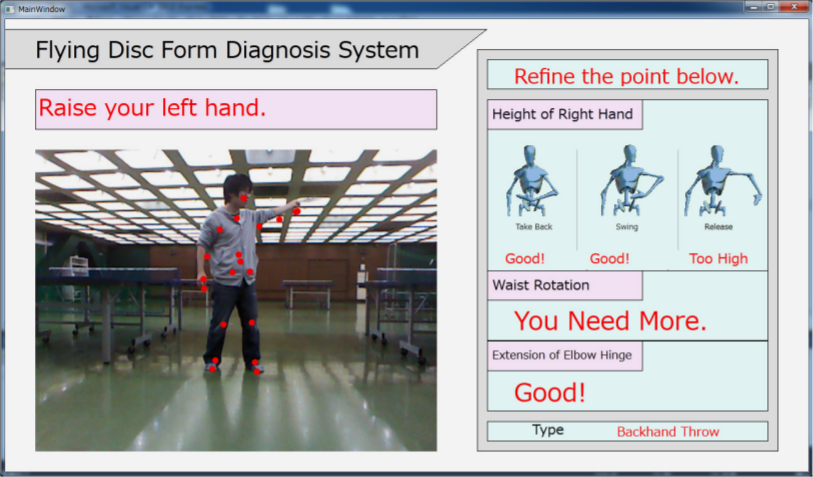
\includegraphics[scale=0.3]{img/flying_disc_TEL.png}
				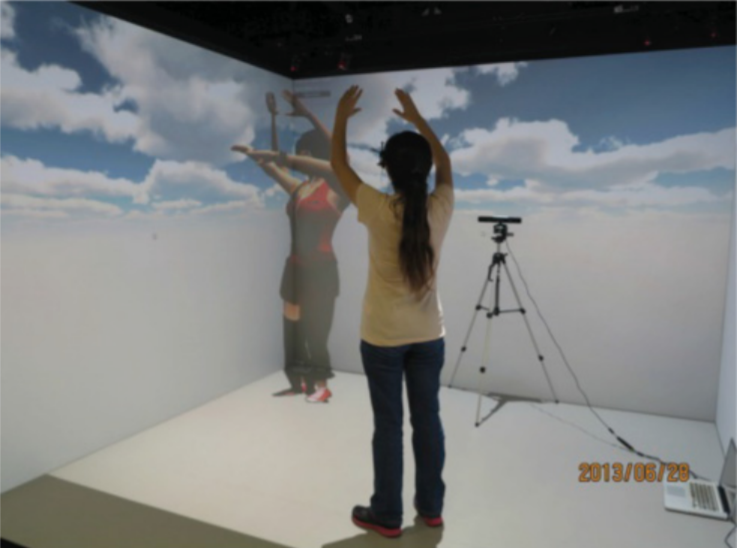
\includegraphics[scale=0.3]{img/dance_cave_TEL.png}
		\end{itemize}
		
				
	\end{frame}
	
	\subsection{Analyse par détection de séquence ordonnée d'actions}
	\begin{frame}{\subsecname}
		\begin{itemize}[label=$\bullet$]
			\item Scénarisation par l'expert, puis reproduction par l'apprenant \mycite{Mahdi2019TaE, Delest2019MaE}	
			
			\vspace{1cm}
			
			\centering
				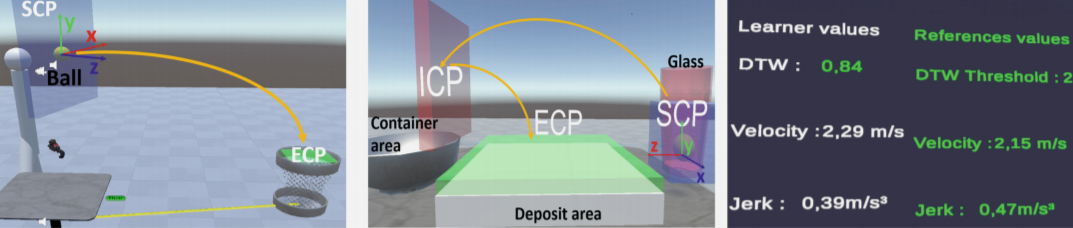
\includegraphics[scale=0.4]{img/Delest_system.png}
		\end{itemize}
	\end{frame}
	
	\subsection{Analyse basée sur des techniques d'apprentissage automatique}
	\begin{frame}{\subsecname}
		\begin{itemize}[label=$\bullet$]
			\item Évaluation de gestes sans \textit{a priori} sur le geste en lui-même \mycite{Pirsiavash2014AQA})
			\item Segmentation, reconnaissance et évaluation de gestes à l'aide d'algorithmes de logique floue \mycite{Patrona2018MaA})
		\end{itemize}
		
		\centering
		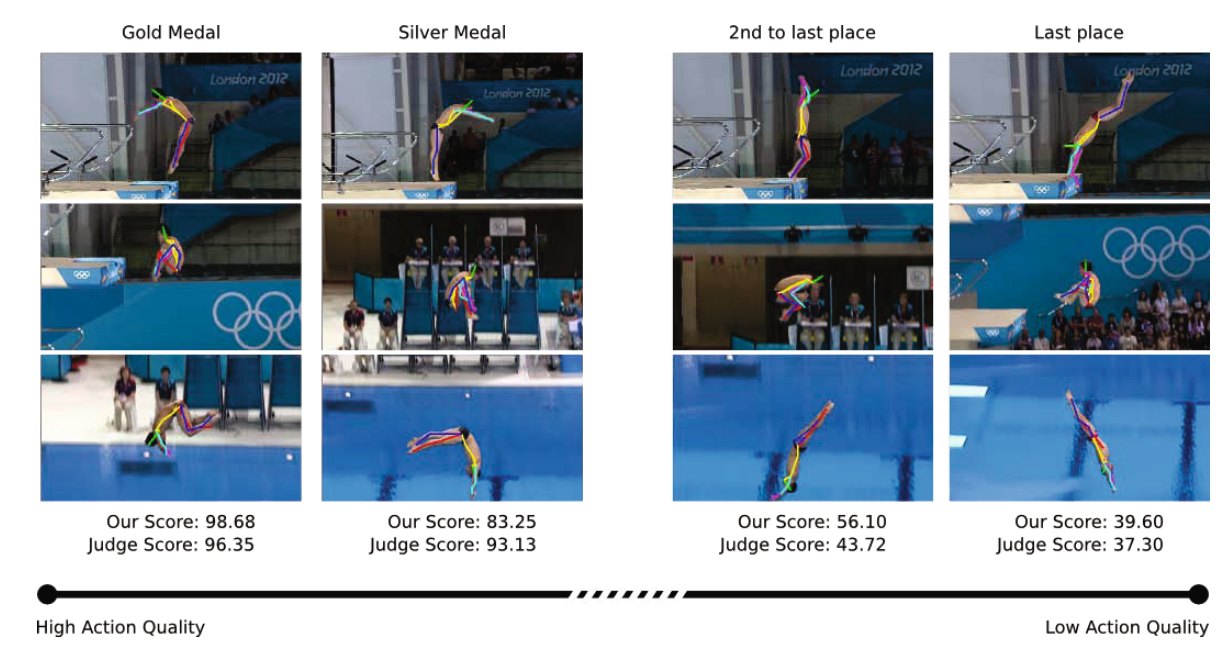
\includegraphics[scale=0.3]{img/olympic_games.png}
	\end{frame}
	
	\subsection{Bilan des systèmes existants}
	\begin{frame}{\subsecname}
		\begin{table}[]
			\resizebox{\textwidth}{!}{%
			\begin{tabular}{c|c|c|c}
			Système basé sur... & Place de l'utilisateur & Objectif & Inconvénients \\\hline
			Analyse humaine & Au centre & \makecell{Fourni des visualisations\\du geste} & \makecell{Difficulté pour non-expert,\\pas d'analyse} \\\hline
			Descripteurs & Variable & \makecell{Fournir des valeurs\\pertinentes} & \makecell{Nécessite des\\connaissances scientifiques} \\\hline
			Séquence d'actions & Variable & \makecell{Segmenter et analyser\\le mouvement} & \makecell{Intégration de la connaissance\\ lors de la conception} \\\hline
			Analyse automatique & Souvent écarté & \makecell{Analyser le geste\\sans présence d'expert} & Absence de l'expert \\
			\end{tabular}
			}
		\end{table}
	\end{frame}
	
	\subsection{Positionnement}
	\begin{frame}{\subsecname}
		\begin{itemize}[label=$\bullet$]
			\item Assistance à l'expert dans sa tâche d'analyse
			\item Système d'évaluation du geste, proposant également des indicateurs visuels pour l'expert
			\item Intégration de la connaissance experte avant l'utilisation en situation d'apprentissage, mais sans de ré-ingénierie nécessaire 
		\end{itemize}
	\end{frame}

	\part{Contributions}
	\section{Motion Learning Analytics}
	\begin{frame}{\secname}
		\begin{block}{Motion Learning Analytics (MLA)}
			\begin{itemize}[label=$\bullet$]
				\item Propose un ensemble d'outils pour pré-traiter et extraire des informations permettant d'analyser un geste
				\item Permet également de comparer les mouvements à ceux d'un expert, à l'aide de techniques de clustering
				\item Propose un ensemble de métriques, ainsi que de visualisation pour assister l'expert dans sa tâche d'évaluation des gestes
			\end{itemize}
		\end{block}
	\end{frame}
	
	\subsection{Architecture MLA}
	\begin{frame}{\subsecname}
	\centering
		\includegraphics[scale=0.3]{img/mla/MLA_color_16.png}
	\end{frame}

	\section{Traitements des données}
	
	\subsection{Matériel de capture}
	\begin{frame}{Perception Neuron}
		\centering
		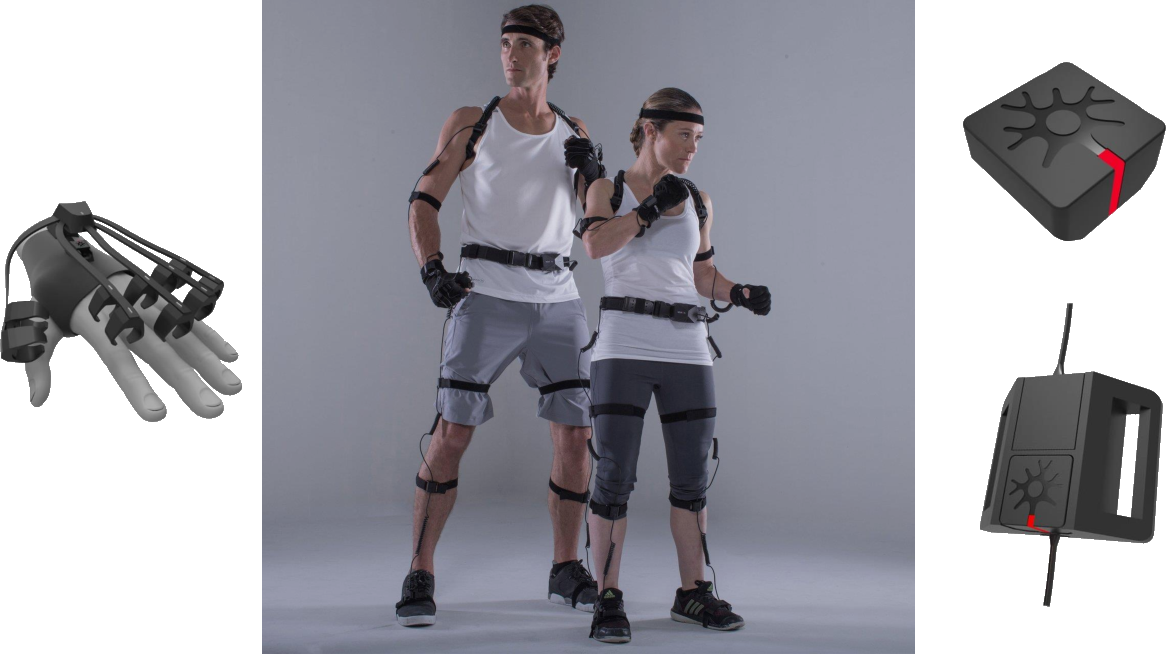
\includegraphics[scale=0.4]{img/Perception_Neuron.png}
	\end{frame}
	
	\subsection{Pré-traitements}
	\begin{frame}{\subsecname}
		\begin{block}{Variation de la taille des membres}
			Fixation de la taille des membres à l'aide de la posture de référence (posture à l'indice 0)
		\end{block}
		
	\begin{block}{Filtrage et extraction du moment d'intérêt}
		\centering
			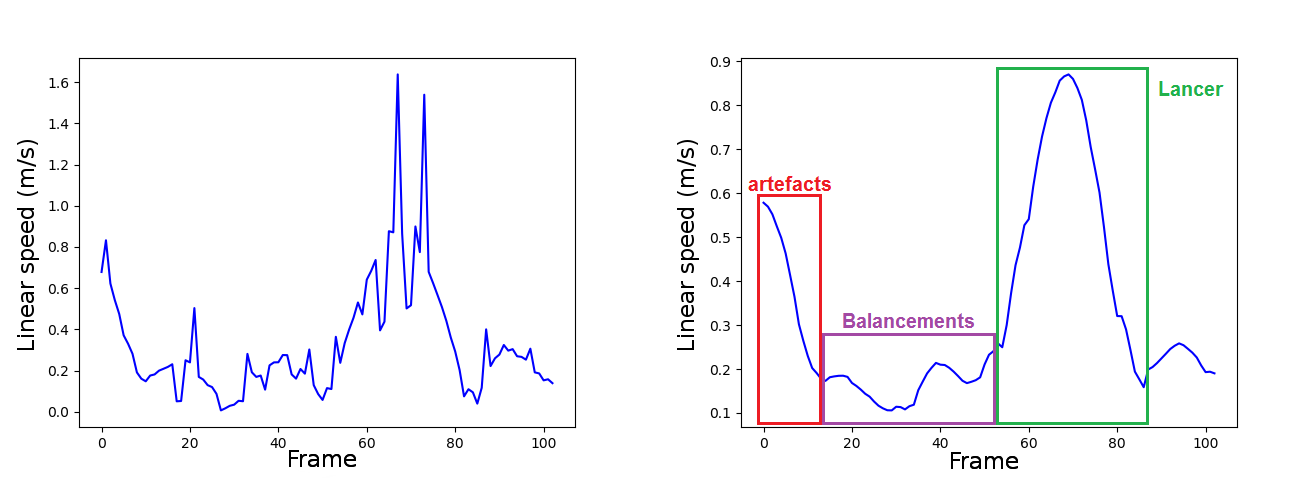
\includegraphics[scale=0.35]{img/before_after_savgol_complete.png}
	\end{block}
		
	\end{frame}
	
	\section{Analyse et représentation visuelle}
	\begin{frame}{\secname}
	Objectif : assister l'expert dans sa tâche d'évaluation du geste, en lui permettant d'obtenir un retour visuel sur les différences entre le geste de l'apprenant et le sien.
	Pré-requis :
	\begin{itemize}[label=$\bullet$]
		\item Données de l'expert réparties en bons gestes / gestes correspondant à un défaut
		\item Données de l'apprenant
		\item Liste de descripteurs à associer aux défauts
	\end{itemize}
	\end{frame}
	
	\begin{frame}{Déroulement}
	\begin{itemize}
		\item \textbf{1.} (Facultatif) Normalisation des données
		\item \textbf{2.} Clustering des données de l'expert à l'aide d'un k-means, afin d'obtenir deux groupes correspondant aux bons et aux mauvais gestes (apprentissage semi-supervisé)
		\item \textbf{3.} Comparaison des données de l'apprenant à celles de l'expert
		\item \textbf{4.} Retour sous forme visuelle (utilisation d'un PCA si dimensionnalité des données > 2)
	\end{itemize}
	
	\end{frame}
	
	\begin{frame}{Étape de clustering}
	\centering
		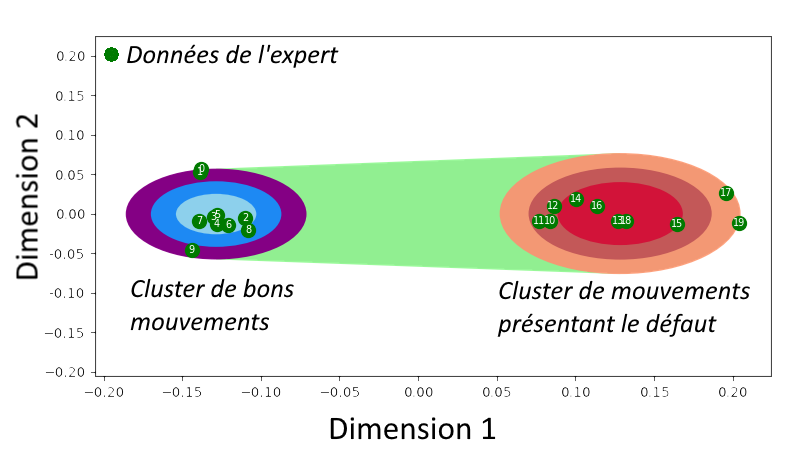
\includegraphics[scale=0.5]{img/feedback_expert_cluster_example.png}
	\end{frame}
	
	\begin{frame}{Étape de comparaison}
	\centering
		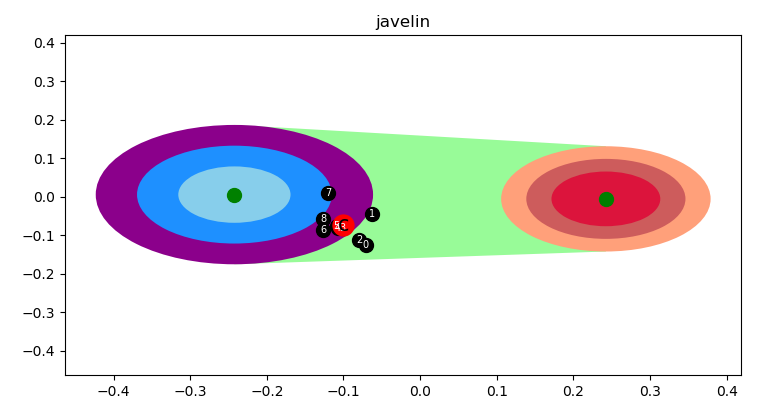
\includegraphics[scale=0.4]{img/feedback_one.png}
	\end{frame}


	\part{Expérimentations}
	\section{Hypothèses de recherche}
	\begin{frame}{\secname}
		\begin{itemize}[label=$-$]
			\item \textbf{H1} : Il est possible de regrouper les gestes selon leurs propriétés cinématiques communes.
			\item \textbf{H2} : Il est possible de séparer les gestes des apprenants en deux groupes correspondant à une dichotomie geste réussi / geste raté afin de déterminer, pour une situation d'apprentissage donnée, les propriétés d'un ensemble fini de gestes réussis.
			\item \textbf{H3} : Il est possible de séparer les gestes en fonction de propriétés attendues et identifiées au préalable par l'expert.
		\end{itemize}
	\end{frame}
	
	\begin{frame}
		\begin{itemize}[label=$-$]
			\item \textbf{H4} : Il est possible de corriger chaque défaut du geste de l'apprenant, en lui indiquant les défauts majeurs à corriger en premier. Un défaut majeur est identifié par la plus grande distance séparant le mouvement courant de l'apprenant, du groupe de gestes acceptables ayant éliminé ce défaut.
			\item \textbf{H5} : L'utilisation du système MLA basée sur l'hypothèse 4 permet d'améliorer l'apprentissage du geste par rapport à une situation sans le système MLA.
			\item \textbf{H6} : L'utilisation du système MLA en tant qu'assistant à l'enseignant permet d'améliorer l'apprentissage du geste par rapport à une situation sans MLA, et à une situation avec MLA et sans enseignant.
		\end{itemize}
	\end{frame}

	\section{Protocole commun}
	\begin{frame}{Protocole commun aux trois expérimentations}
		\begin{itemize}[label=$\bullet$]
			\item Instructions données à l'apprenant
			\item Mesure selon les préconisations de NOITOM
			\item Calibrations de la combinaison d'acquisition de mouvement
			\item familiarisation avec la combinaison 
		\end{itemize}
	
		\centering
		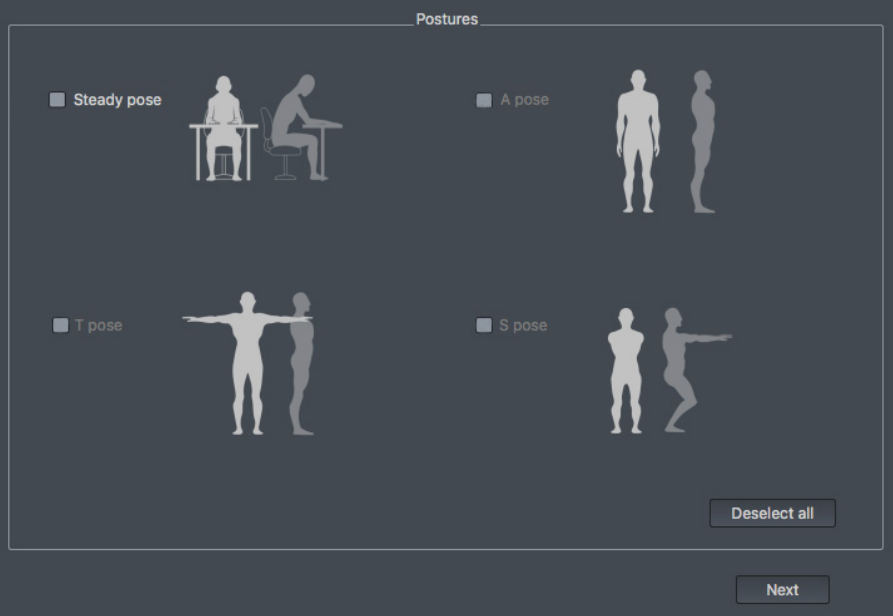
\includegraphics[scale=0.3]{img/percpetion_neuron_calibrations.png}
	\end{frame}
	
	\subsection{Workflow du système MLA}
	\begin{frame}{\subsecname}
	\centering
		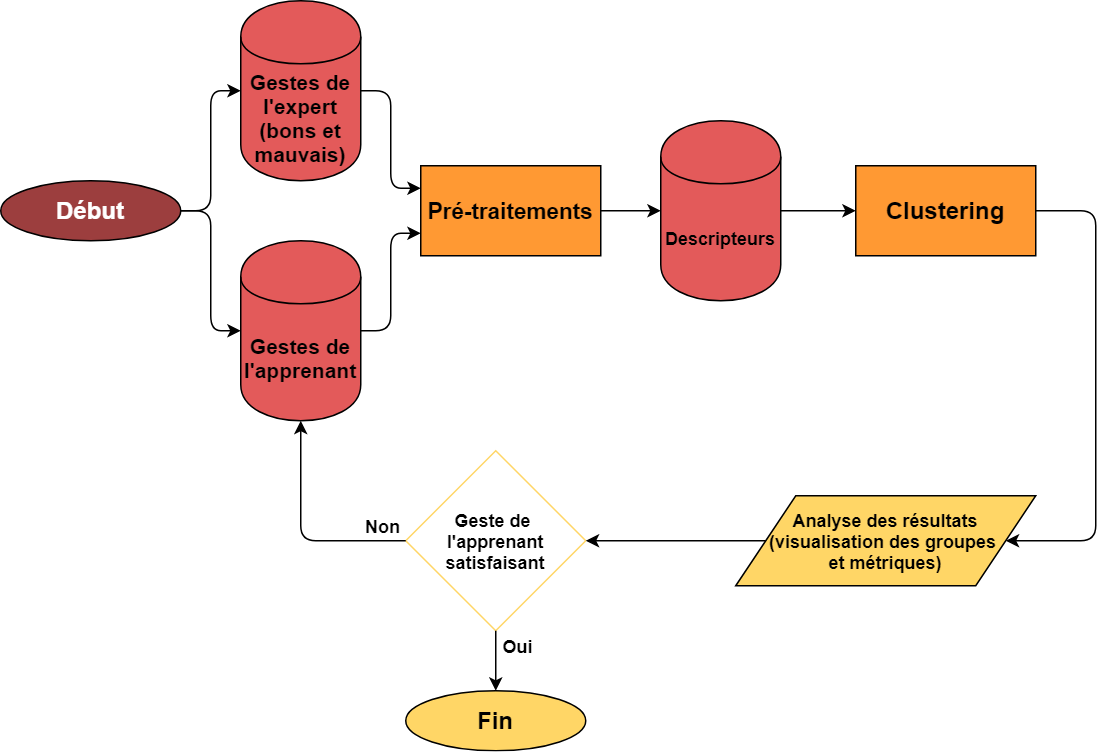
\includegraphics[scale=0.3]{img/workflow_MLA.png}
	\end{frame}
	
	\section{Métriques calculées}
	\begin{frame}{\secname : Average Silhouette Score (\textit{ASS})}
		\begin{block}{Silhouette Score}
			Calcule la bonne appartenance d'un point au cluster qui lui est assigné, en calculant la distance de ce point à tous les autres contenus dans le même cluster par rapport à ceux des autres clusters.
		\end{block}
		
		\begin{block}{Average Silhouette Score \mycite{Rousseeuw1987Sag}}
			Moyenne des Silhouette Score de chaque point de donnée.
		\end{block}
	\end{frame}
	
	\begin{frame}{Average Silhouette Score (\textit{ASS})}
		\begin{itemize}[label=$\bullet$]
			\item $[0;0.25]$ : aucune structure n’est discernable au sein des données
			\item$ ]0.25; 0.5]$ : il existe une structure, bien que mal définie, voire artificielle
			\item $]0.5;0.70
			]$ : une structure existe au sein des données (séparation correcte des clusters)
			\item $]0.7;1]$ : une structure est clairement définie au sein des données (très bonne séparation des clusters)
		\end{itemize}
	\end{frame}
	
	\begin{frame}{\secname : Adjusted Rand Index (\textit{ARI})}
		\begin{block}{Adujsted Rand Index \mycite{Morey1984ARI}}
			Mesure de similarité entre deux partitionnements de données différents. Cette mesure est un ajustement du Rand Index \mycite{Rand2971RI}. Une valeur de 1 indique une correspondance parfaite entre les deux partitionnement, alors qu'une valeur de 0 indique une affectation aléatoire des données. La normalisation induite par l'ajustement peut produire des valeurs négatives \mycite{Meila2007Cca}. 
		\end{block}
	\end{frame}

	\section{Lancer de balle}
	\subsection{Objectifs et principe}
	\begin{frame}{\secname : \subsecname}
		\begin{block}{Objectif}
			Vérifier si le système est capable de séparer les gestes selon un étiquetage vérifiable par un humain à l'aide des descripteurs et des algorithmes choisis (\textbf{H1}, \textbf{H2}).
		\end{block}
		
		\vspace{1cm}
		
		\centering
		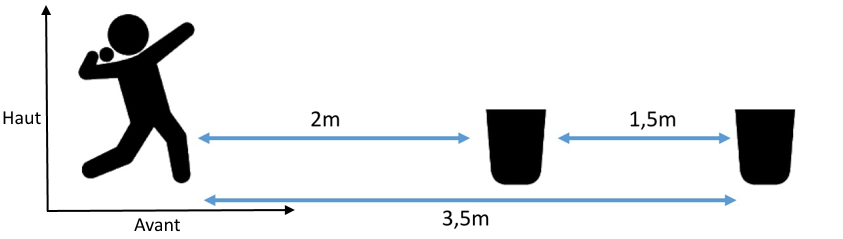
\includegraphics[scale=0.5]{img/ball_throwing.png}

	\end{frame}
	
	\subsection{Résultats}
	\begin{frame}{\subsecname : \subsecname}
		\begin{block}{Participants}
			\begin{itemize}[label=$\bullet$]
				\item 2 participants
				\item 100 lancers par personne
			\end{itemize}
		\end{block}
		
	Algorithme utilisé : k-means, avec $k=2$.
	\begin{itemize}
		\item Séparation correcte des clusters (norme du vecteur vitesse de la main et vecteurs vitesses en x, y et z ($ASS \approx 0.6$)) / \textbf{H1} validée dans le contexte de cette expérimentation
		\item Séparation correspondant à l'étiquetage « type de lancer » ($ARI \approx 0.85$)
		\item Séparation ne correspondant pas au degré de réussite du geste : \textbf{H2} non validée
	\end{itemize}
		
		
	\end{frame}


	\section{Bottle Flip Challenge}
	\subsection{Objectifs et principe}
	\begin{frame}{\secname : \subsecname}
		\begin{block}{Objectif}
			 Déterminer s'il est possible d'obtenir une séparation des données en deux clusters, correspondant au degré de réussite du geste. ( \textbf{H2}).
		\end{block}
	
		\centering
		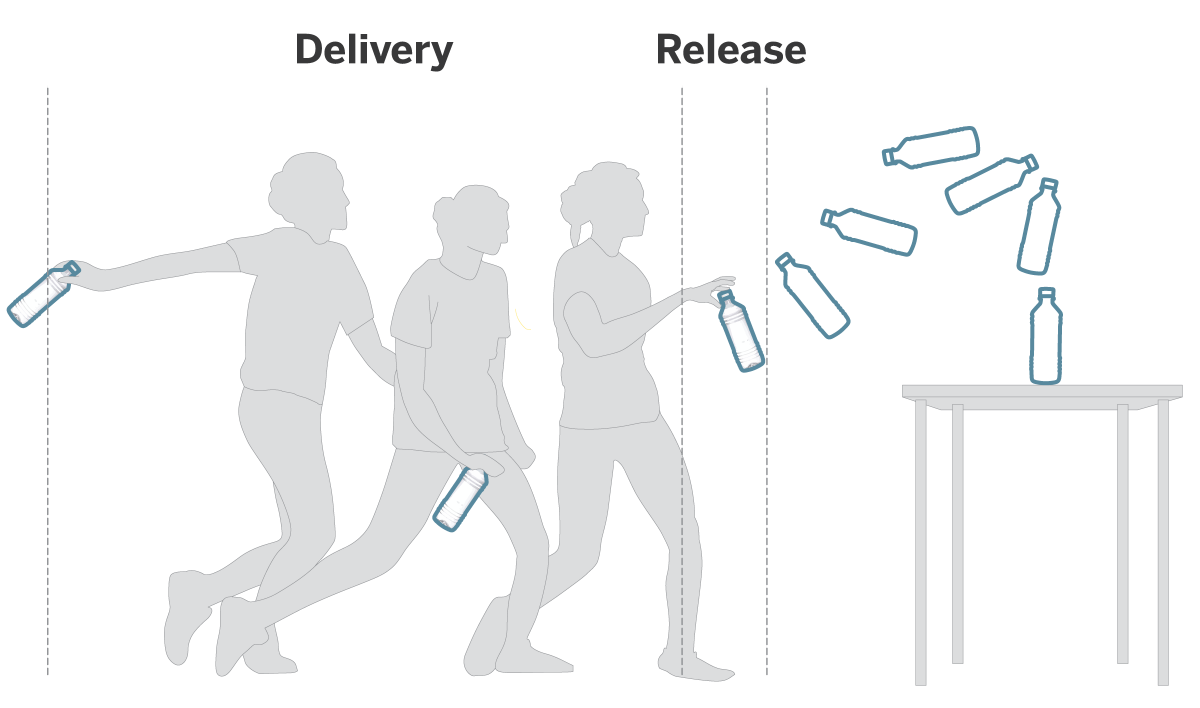
\includegraphics[scale=0.2]{img/BFC_example.png}
	\end{frame}
	
	\subsection{Résultats}
	\begin{frame}{\secname : \subsecname}
		\begin{block}{Participants}
			\begin{itemize}[label=$\bullet$]
				\item 13 participants (2 gauchers, 11 droitiers)
				\item 100 lancers par personne
			\end{itemize}
		\end{block}

		Algorithme utilisé : k-means, avec $k=2$.
		\begin{itemize}
			\item Séparation correcte des clusters pour les vecteurs vitesse en x, y et z des droitiers ($ASS \approx 0.75$)
			\item Séparation ne correspondant pas au degré de réussite du geste ($ARI \approx 0$): \textbf{H2} non validée
		\end{itemize}
		
	\end{frame}

	\section{Lancer de fléchettes}
	\subsection{Objectifs et principe}
	\begin{frame}{\secname : \subsecname}
		\begin{block}{Objectifs}
			\begin{itemize}[label=$\bullet$]
				\item Montrer qu'il est possible, à l'aide du système de retours à l'apprenant basé sur les démonstrations de l'expert et l'estimation de valeurs d'acceptabilité empiriques des propriétés du geste, de donner des conseils pertinents lors de la réalisation de ces derniers (\textbf{H3}, \textbf{H4})
			 	\item Montrer qu'une amélioration du geste, en termes de précision du tir et de la « forme » du mouvement résultait de ces conseils (\textbf{H5})
			 	\item Évaluation en terme d'usage de l'efficacité du système selon les modalités précédemment citées : utilisation du système seul, ou utilisation conjointe avec l'analyse de l'expert (\textbf{H6})
			 \end{itemize}
		\end{block}
	
		\begin{block}{Principe}
			Lancer de fléchettes (sport)
		\end{block}
		
	\end{frame}
	
	\subsection{Position de tir}
	\begin{frame}{\secname : \subsecname}
		\centering
		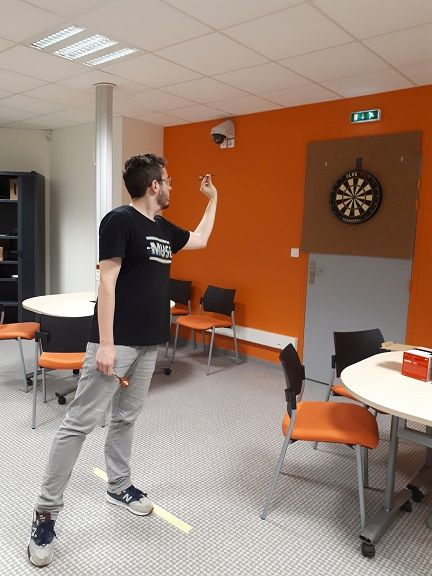
\includegraphics[scale=0.3]{img/darts_position_alt.jpg}
	\end{frame}

	\subsection{Schéma de l'installation}
	\begin{frame}{\secname : \subsecname}
		\centering
		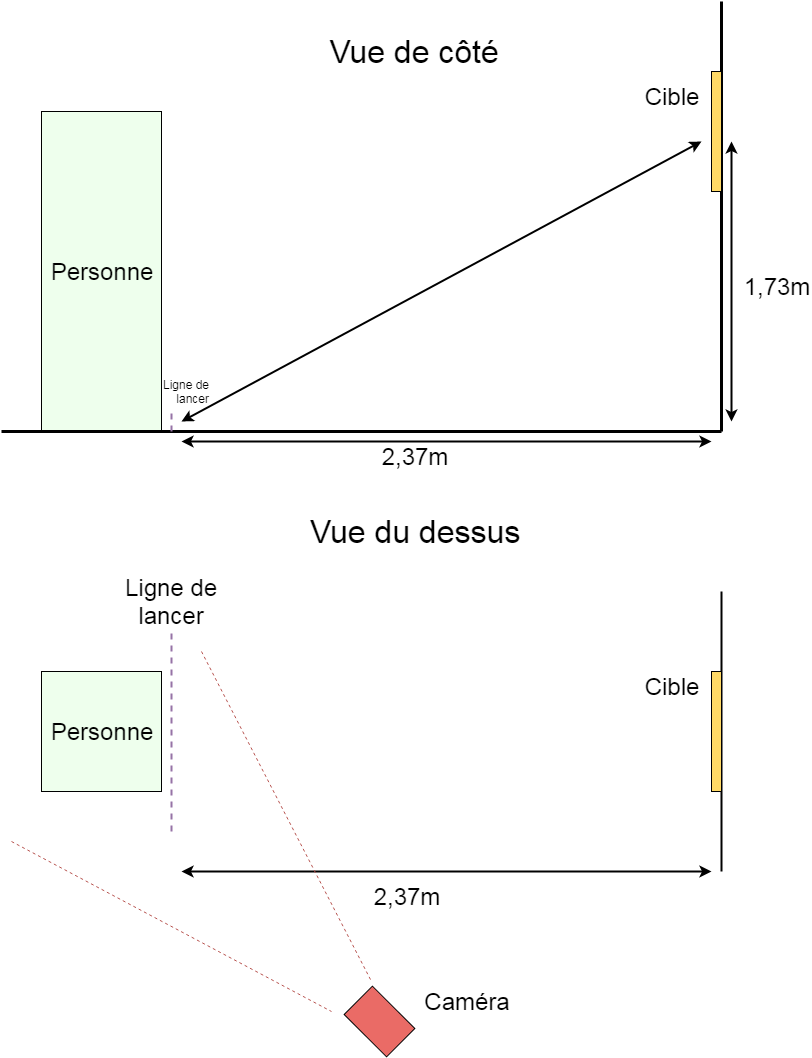
\includegraphics[scale=0.2]{img/Darts_scheme.png}
	\end{frame}
	
	\subsection{Acquisition des données de l'expert et participants}
	\begin{frame}{\secname : \subsecname}
		\begin{block}{Acquisition des données de l'expert}
			\begin{itemize}
				\item \textbf{1.} Identification des défauts quantifiables
				\item \textbf{2.} Capture de mouvements de lancers corrects réalisés par l'expert
				\item \textbf{3.} Pour chaque défaut, capture de mouvements de lancers par l'expert présentant ce défaut 
			\end{itemize}
		\end{block}
	
		\begin{block}{Participants}
			\begin{itemize}[label=$\bullet$]
				\item 45 participants, répartis en 3 groupes de 15 personnes :
				\begin{itemize}
					\item \textbf{Groupe 1} : Conseils de l'expert seulement
					\item \textbf{Groupe 2} : Conseils du système seulement
					\item \textbf{Groupe 3} : Expert s'appuyant sur le système pour donner ses conseils
				\end{itemize}
				\item 36 lancers par personne ($4 \times 9$ lancers)
			\end{itemize}
		\end{block}
	\end{frame}
	
	\subsection{Défauts}
	\begin{frame}{\subsecname}
		\centering
		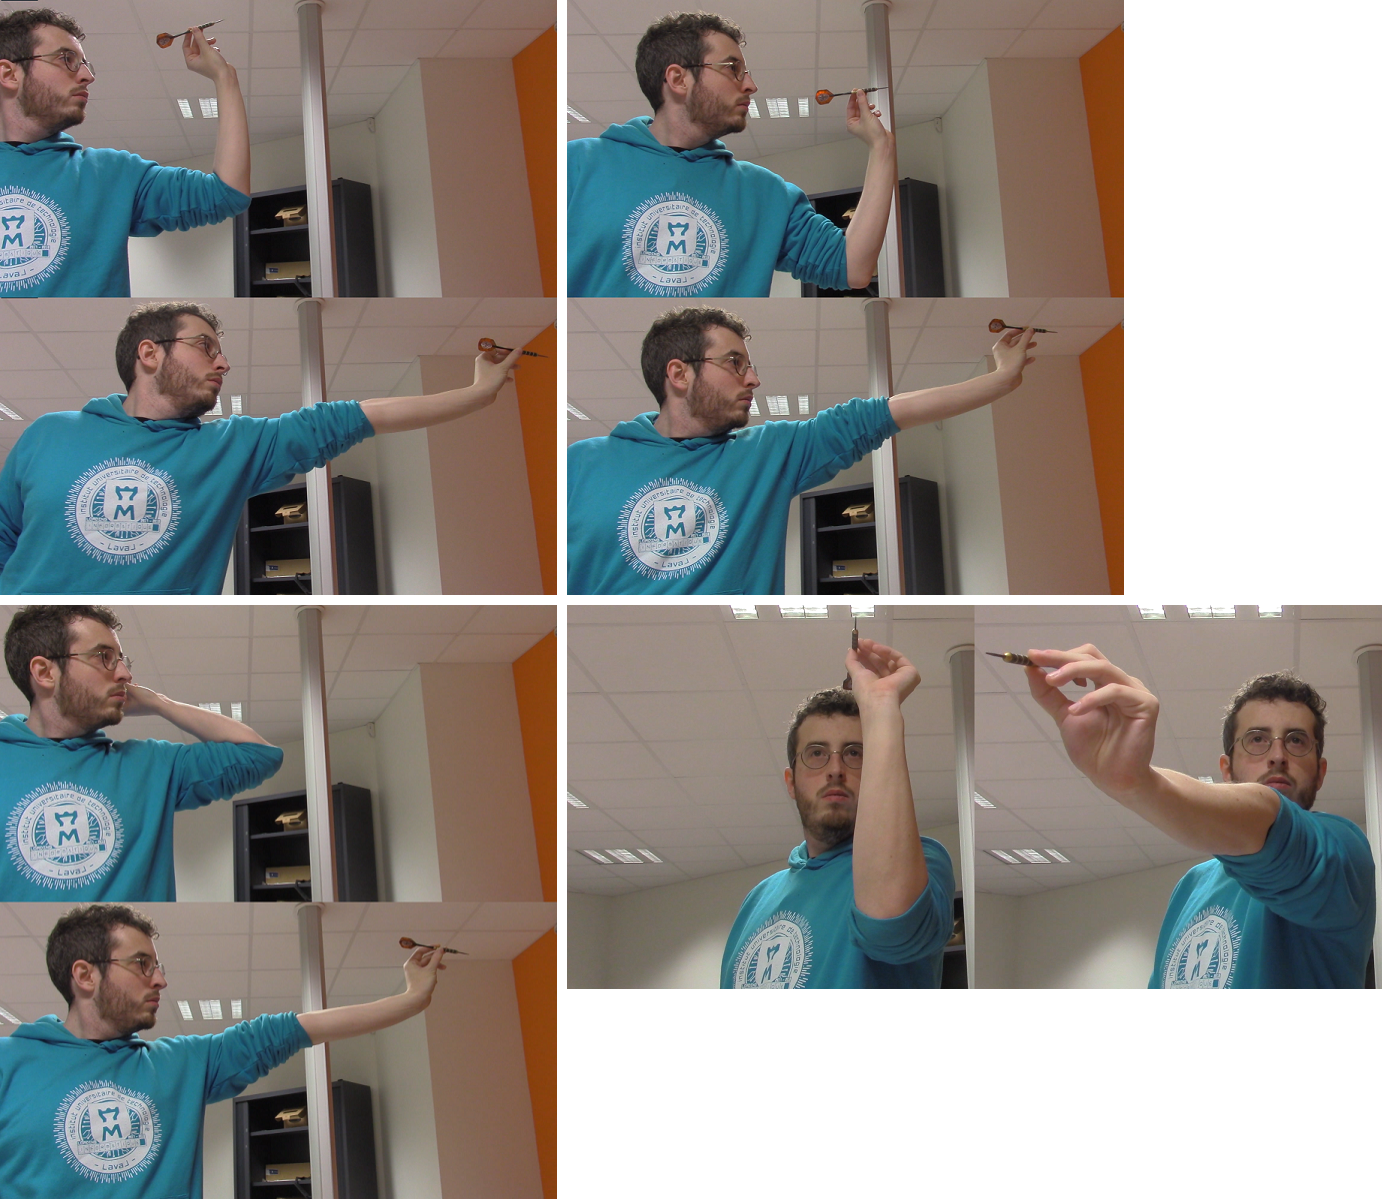
\includegraphics[scale=0.3]{img/all_defaults.png}
	\end{frame}
	
	\subsection{Données utilisées}
	\begin{frame}{\secname : \subsecname}
		\begin{block}{Descripteurs}
			\begin{itemize}[label=$\bullet$]
				\item Leaning : vitesse moyenne des deux épaules
				\item Elbow move : vitesse moyenne de coude et de l'épaule du côté de la préférence manuelle de la personne
				\item Javelin : distance en x, y et z de la main par rapport à la tête
				\item Align arm : moyenne de la largeur, ainsi que de l'écart-type, de la boîte englobante allant de la main à l'épaule du côté de la préférence manuelle de la personne
			\end{itemize}
		\end{block}
	\end{frame}
	
	\subsection{Déroulement}
	\begin{frame}{\secname : \subsecname}
		\begin{itemize}[label=$\bullet$]
			\item Pré-questionnaire : taille, niveau d'expertise auto-évalué aux fléchettes (échelle de Likert à 7 réponses), ainsi que toute pratique actuelle d'un sport
			\item Début de l'expérimentation
			\item 9 lancers, suivit de deux conseils, 4 fois d'affilé
			\item Post-questionnaire : ressenti de la personne par rapport à la combinaison, à la progression de son geste et à l'auto-évaluation de sa performance
		\end{itemize}
		
	\end{frame}
	
	\subsection{Résultats}
	\begin{frame}{\subsecname : Questionnaires}
	\centering
		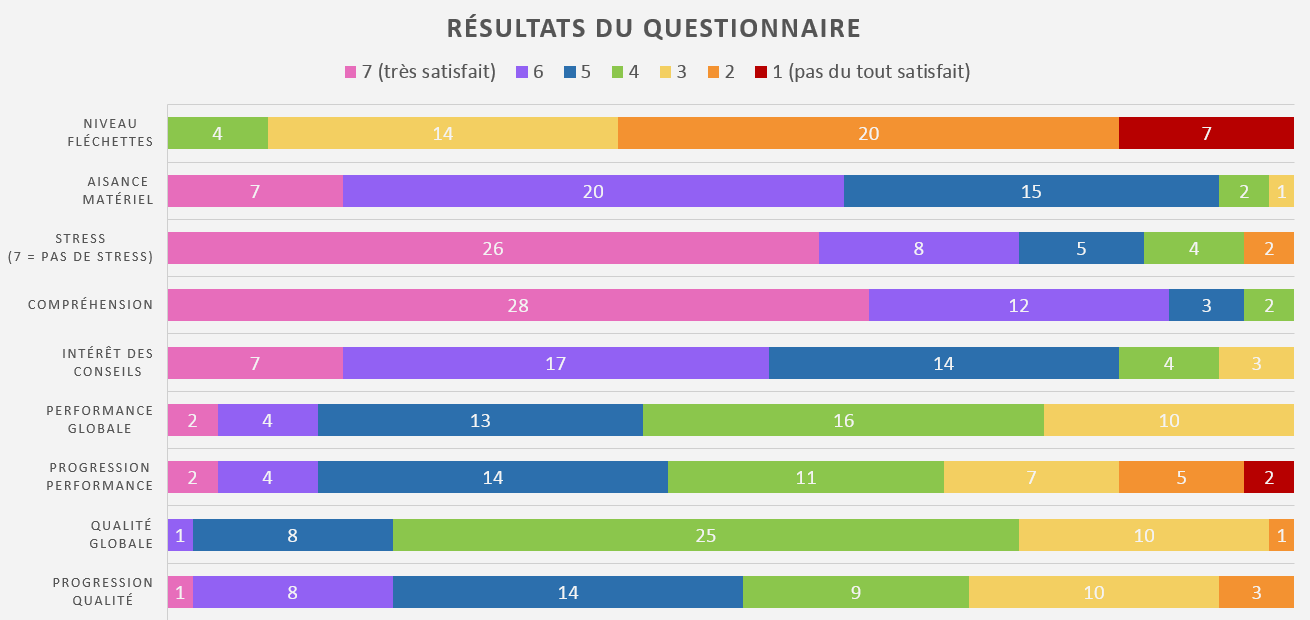
\includegraphics[scale=0.4]{img/graph_questionnaires.png}
	\end{frame}		
	
	\begin{frame}{\secname : \subsecname}
	Algorithme utilisé : k-means, avec $k=2$.
	
	\begin{table}[h]
		\centering
		\begin{tabular}{c|c|c}
			& Silhouette Score & Adjusted Rand Index\\\hline
			Leaning & 0.85 & 1\\
			Elbow move & 0.58 & 0.47\\
			Javelin & 0.79 & 1\\
			Align arm & 0.53 & 1\\
		\end{tabular}
	\end{table}
		
		Hypothèse \textbf{H3} validée dans le contexte de cette expérimentation
		
	\end{frame}
	
	\begin{frame}{\secname : \subsecname}
		\begin{block}{Évaluation}
			Deux approches, en intergroupe et en intragroupe :
			\begin{itemize}[label=$\bullet$]
				\item Amélioration de l'objectif du mouvement (distance par rapport au centre de la cible)
				\item Amélioration des propriétés du mouvement (rapprochement du centroïde des données de l'apprenant au bon cluster de l'expert)
			\end{itemize}
		\end{block}
	\end{frame}
	
	\begin{frame}{\secname : \subsecname}
		En premier lieu, test de normalité : Shapiro-Wilk et d'Agostino-Pearson
		\begin{table}[]
			\begin{adjustbox}{max width=\textwidth}
			\begin{tabular}{l|l|l}
				Type de distribution & Normale & Non-normale \\\hline
				Intergroupe & ANOVA & Kruskal-Wallis \\
 				& Levene & Wilcoxon-Mann-Whitney \\
 				& Student paire-à-paire &  \\\hline
				Intragroupe & Student sur deux échantillons & Rangs signés de Wilcoxon
			\end{tabular}
			\end{adjustbox}
		\end{table}
	\end{frame}
	
	\begin{frame}{\secname : \subsecname}
		Amélioration significatives en intragroupe entre les jeu 1 et 4 : \textit{leaning} et \textit{elbow move} pour tous les groupes, \textit{javelin} et \textit{align arm} pour le groupe 2 : \textbf{H4} est validée pour le groupe 2, et partiellement validée pour les autres groupes\\
		\vspace{1cm}
		Pas d'amélioration significatives en intergroupe : \textbf{H5} et \textbf{H6} ne sont pas validées
		
	\end{frame}
	
	\subsection{Limites}
	\begin{frame}{\secname : \subsecname}
		\begin{itemize}[label=$\bullet$]
			\item Phénomène d'auto-correction de l'expert
			\item Nombre de lancers pour les apprenants faibles (36)
			\item Pause entre chaque série de 9 lancers : perte du geste
			\item Systématiquement 2 conseils donnés
			\item Analyse de l'expert seul plus difficile dans le cadre de l'expérimentation
			\item Dans une situation d'apprentissage réelle, données extérieures au mouvement de l'apprenant
			\item L'évaluation du système suppose une prise en compte des conseils donnés
		\end{itemize}
	\end{frame}
	
	\part{Synthèse des contributions et perspectives}
	\section{Synthèse des contributions}
	
	\begin{frame}{\secname}
		\begin{itemize}[label=$\bullet$]
			\item Proposition d'un EIAH dédié à l'apprentissage des gestes
			\item Permet le pré-traitement des données, l'extraction de descripteurs et l'analyse du mouvement de l'apprenant
			\item Généricité pensée dès la conception
			\item Expérimentations menées pour valider les différents aspects du système
		\end{itemize}
	\end{frame}
	
	\section{Limites des travaux présentés}
	\begin{frame}{\secname}
		\begin{itemize}[label=$\bullet$]
			\item Manque d'interface graphique pour utiliser le système
			\item Pertinence des indicateurs visuels à analyser
			\item L'utilisation du Perception Neuron pour la captation implique l'utilisation de techniques de filtrage pour les données
			\item Dans le cadre de l'expérimentation du lancer de fléchettes, faible nombre de lancers
		\end{itemize}
	\end{frame}
	
	\section{Perspectives}
	\begin{frame}{\secname : explication des données non-alignées}
		Si dimensionnalité > 2, PCA : perte de sémantique
		
		\centering
			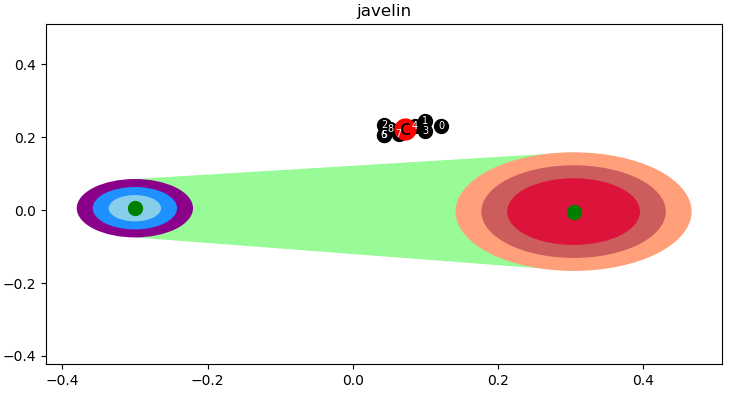
\includegraphics[scale=0.5]{img/non_aligned_default.png}
	\end{frame}
	
	\begin{frame}{\secname : création de nouveaux descripteurs}
		Système basé sur des patrons de conception :
		
		\begin{framed}
		DESCRIPTOR Hauteur hanche: POSITION\_ALL[2]
		\end{framed}
		pour la hauteur de la hanche (valeur en \textit{y}) calculée sur tout le mouvement.\\

		\begin{framed}
		DESCRIPTOR Vitecceleration: SPEED\_ALL[2] + ACCELERATION\_ALL[1]
		\end{framed}
		pour calculer l'addition de la composante en $y$ de la vitesse et de la composante en $x$ de l'accélération.\\
	\end{frame}
	
	\begin{frame}{\secname : clustering récursif}
		\centering
		\includegraphics[scale=0.5]{img/subclustering/init2.png}
	\end{frame}


\end{document}







